\chapter{तापीय विकिरण}\label{ch:b2:thermal-radiation}

हर गरम चीज़ दमकती है। कोई हाथ, कोई दीवार, कमरे के ताप पर पानी का कोई
गिलास अदृश्य रूप से विकिरित करते हैं, \qty{10}{\micro m} के पास के
तरंगदैर्घ्यों पर, प्रति वर्ग मीटर कुछ सौ वाट; किसी सलाख को गरम कीजिए और
\qty{600}{\celsius} पर वह धुँधली लाल दमकती है, \qty{1000}{\celsius} पर
नारंगी, और \qty{2500}{\celsius} पर --- किसी बल्ब का तंतु --- सफ़ेद; और
\qty{5800}{K} पर सूर्य की सतह पीली-सफ़ेद, प्रति वर्ग मीटर साठ मेगावाट,
विकिरित करती है, और वही प्रकाश, आठ मिनट की यात्रा के बाद, पृथ्वी को उस ताप
पर थामे रखता है जहाँ पानी द्रव है। विकिरण ऊष्मा-अंतरण का तीसरा ढंग है और
अकेला ऐसा जो ख़ाली आकाश पार करता है; वही वह जगह भी है जहाँ चिरसम्मत भौतिकी
हार गई और प्लांक को, 1900 में, क्वांटम लाना पड़ा। यह अध्याय उनका खोजा नियम
बताता है, उससे वे दो परिणाम निकालता है जो लगातार काम आते हैं ---
वीन का विस्थापन और श्टेफ़ान--बोल्ट्समान नियम --- और उन्हें पिंडों के बीच के
विनिमयों पर, सूर्य तथा पृथ्वी पर, और \omterm{prop:b2:thermal-radiation:greenhouse}{हरितगृह प्रभाव} के उस एक-परत प्रतिरूप
पर लगाता है जो हमारी जलवायु तय करता है।

\begin{omfigure}
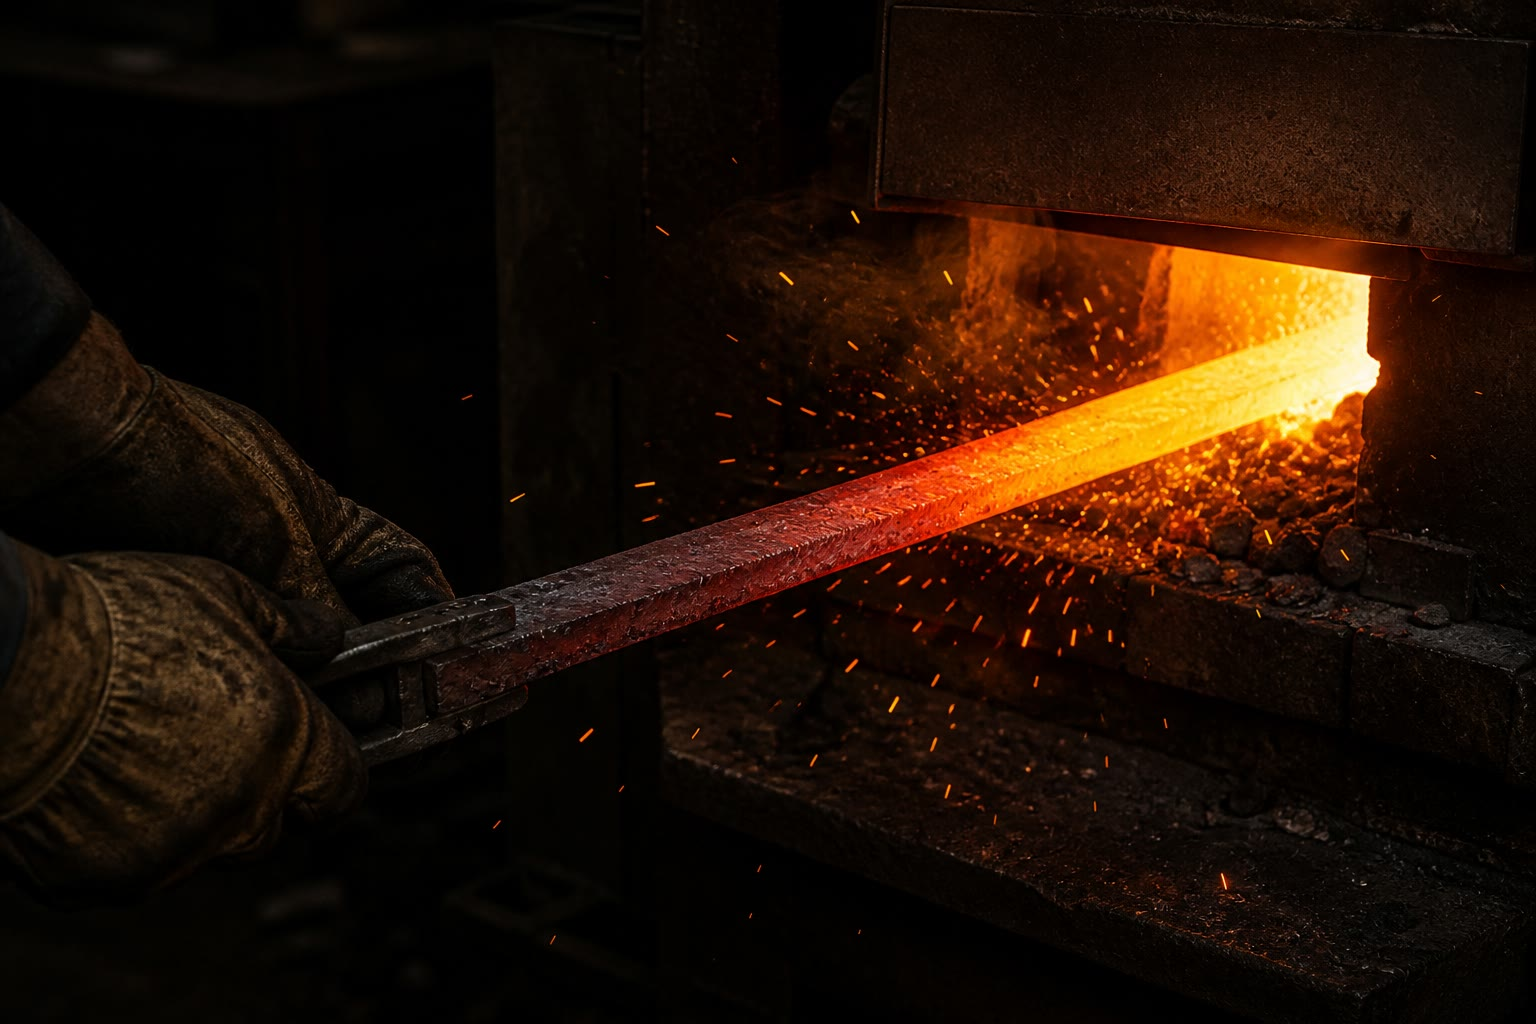
\includegraphics[width=0.58\linewidth]{images/book4/ai/b4-26-glowing-steel-forge.jpg}

{\small भट्ठी पर इस्पात: दमक का रंग --- धुँधला लाल, नारंगी,
पीला, सफ़ेद --- कोई तापमापी है, क्योंकि \omterm{def:b2:thermal-radiation:blackbody}{तापीय विकिरण} का वर्णक्रम
अकेले ताप पर निर्भर करता है।}
\end{omfigure}

\section{तापीय विकिरण और कृष्णिका}

\begin{definition}[तापीय विकिरण, अवशोषकता, कृष्णिका]\label{def:b2:thermal-radiation:blackbody}
ताप $T$ पर हर पिंड अपने आवेशों की तापीय उथल-पुथल से विद्युत्चुंबकीय
विकिरण उत्सर्जित करता है: अर्थात् उसका \emph{तापीय
विकिरण}\index{तापीय विकिरण}। उसकी सतह अपने परिवेश से विकिरण पाती भी है
और उसका कोई अंश $\alpha$ सोख लेती है
(\emph{अवशोषकता}, $0$ और $1$ के बीच, जो आम तौर पर
तरंगदैर्घ्य पर निर्भर करती है), और बाक़ी परावर्तित या पारगत कर देती है। कोई \emph{कृष्णिका}\index{कृष्णिका}
सब कुछ सोख लेती है (हर तरंगदैर्घ्य पर $\alpha = 1$)। किसी बंद कोटर की
दीवार में कोई छोटा छेद व्यावहारिक कृष्णिका है: उसमें घुसता विकिरण
बाहर की राह पाने से पहले ही दीवारों पर सोख लिया जाता है।
\end{definition}

\begin{proposition}[साम्य विकिरण और किरखोफ़ का नियम]\label{prop:b2:thermal-radiation:kirchhoff}
किसी बंद कोटर के भीतर, जिसकी दीवारें $T$ पर हों, विकिरण दीवारों के साथ
साम्य में और \emph{सार्वभौम} है: समदैशिक,
अध्रुवित, और ऐसे वर्णक्रमी ऊर्जा घनत्व $u_\nu(T)$ के साथ (प्रति एकांक
आयतन और एकांक आवृत्ति ऊर्जा) जो केवल $T$ और $\nu$ पर निर्भर करता है, न कि
कोटर के पदार्थ या आकार पर। ऐसे किसी कोटर के छोटे छेद से निकलता विकिरण
$T$ पर \emph{\omterm{def:b2:thermal-radiation:blackbody}{कृष्णिका} विकिरण} है। कोई सतह जो पाए गए विकिरण का अंश
$\alpha_\nu$ सोखती हो, आवृत्ति $\nu$ पर, उसी आवृत्ति पर उसका अंश
$\varepsilon_\nu = \alpha_\nu$ उत्सर्जित करती है जो उसी ताप पर कोई \omterm{def:b2:thermal-radiation:blackbody}{कृष्णिका}
उत्सर्जित करती (अर्थात् उसकी \emph{उत्सर्जकता}\index{उत्सर्जकता}):
\emph{अच्छे अवशोषक अच्छे उत्सर्जक होते हैं}।
\end{proposition}

\begin{proof}
सार्वभौमिकता: एक ही $T$ के दो कोटरों को किसी ऐसे छेद से जोड़िए जिसमें कोई
छन्ना एक ही आवृत्ति जाने दे; यदि घनत्व अलग होते, तो बराबर तापों पर ऊर्जा
एक से दूसरे को बहती, जो दूसरा नियम तोड़ देती। किरखोफ़: सतह को
कोटर में उसके अपने $T$ पर रखिए; साम्य में उसे हर आवृत्ति पर ठीक उतना ही
उत्सर्जित करना पड़ता है जितना वह सोखती है,
$\varepsilon_\nu u_\nu = \alpha_\nu u_\nu$।
\end{proof}

\section{प्लांक का नियम}

\begin{theorem}[प्लांक का नियम]\label{thm:b2:thermal-radiation:planck}
ताप $T$ पर \omterm{def:b2:thermal-radiation:blackbody}{कृष्णिका} विकिरण का वर्णक्रमी ऊर्जा घनत्व
है
\[
u_\nu(T) = \frac{8\pi h\nu^3}{c^3}\,\frac{1}{\eu^{h\nu/k_BT} - 1},
\]
और किसी काली सतह से प्रति एकांक क्षेत्रफल तथा प्रति एकांक
तरंगदैर्घ्य विकिरित शक्ति (उसका \emph{वर्णक्रमी निर्गम}\index{वर्णक्रमी निर्गम}) है
\[
M_\lambda(T) = \frac{2\pi hc^2}{\lambda^5}\,\frac{1}{\eu^{hc/\lambda k_BT} - 1}.
\]
दो सीमाएँ: $h\nu \ll k_BT$ के लिए, $u_\nu \approx 8\pi\nu^2 k_BT/c^3$
(रैले--जीन्स: कोटर की हर विधा चिरसम्मत ऊर्जा
$k_BT$ ले चलती है --- और वह नियम अनंत तक समाकलित होता है, यानी ``पराबैंगनी
विपदा''); और $h\nu \gg k_BT$ के लिए, $u_\nu \approx (8\pi h\nu^3/c^3)
\eu^{-h\nu/k_BT}$ (वीन: ऊर्जा $h\nu$ के किसी फ़ोटॉन का बोल्ट्समान गुणक,
\cref{ch:b2:boltzmann-factor})।
\end{theorem}

\begin{proof}
स्वीकृत: कोटर की विधाओं की गिनती (प्रति एकांक आयतन और आवृत्ति
$8\pi\nu^2/c^3$, दो ध्रुवण) वर्ष 3 के खंड की है,
और किसी विधा की माध्य ऊर्जा, $h\nu/(\eu^{h\nu/k_BT} - 1)$,
चिरसम्मत $k_BT$ के बजाय, क्वांटम उपधारणा है: ऊर्जा
विधा के साथ क्वांटा $h\nu$ में बदली जाती है, जिससे $h\nu \gg k_BT$ वाली विधाएँ
जम जाती हैं। और संबंध $M_\lambda\,\dd\lambda = (c/4)\,u_\nu\,\dd\nu$ वही
ज्यामितीय गुणक है जो \cref{thm:b2:thermal-radiation:stefan} में निकाला गया है।
\end{proof}

\begin{omfigure}
\begin{tikzpicture}
  \begin{axis}[omaxis, width=9.2cm, height=5.2cm, xmin=0, xmax=3.1, ymin=0, ymax=1.12,
    xlabel={$\lambda$ (\unit{\micro m})}, ylabel={$M_\lambda$ (मनमाने एकांक)}, xtick={0.5,1,1.5,2,2.5,3}, ytick=\empty, clip=false,
    legend style={font=\scriptsize, at={(0.97,0.95)}, anchor=north east, draw=none, fill=none}]
    \fill[yellow!40, opacity=0.6] (axis cs:0.4,0) rectangle (axis cs:0.7,1.08);
    \addplot[omDef, thick, domain=0.2:3.1, samples=160] {9.25*x^(-5)/(exp(14388/(x*5000))-1)};
    \addlegendentry{\qty{5000}{K}}
    \addplot[omThm, thick, domain=0.25:3.1, samples=160] {9.25*x^(-5)/(exp(14388/(x*4500))-1)};
    \addlegendentry{\qty{4500}{K}}
    \addplot[omExo, thick, domain=0.3:3.1, samples=160] {9.25*x^(-5)/(exp(14388/(x*4000))-1)};
    \addlegendentry{\qty{4000}{K}}
    \node[font=\scriptsize, anchor=south] at (axis cs:0.55,1.08) {दृश्य};
  \end{axis}
\end{tikzpicture}

{\small तीन तापों पर प्लांक का वर्णक्रम: चोटी $1/T$ की तरह छोटे
तरंगदैर्घ्यों की ओर चलती है (वीन) और क्षेत्रफल $T^4$ की तरह बढ़ता है
(श्टेफ़ान)। केवल सबसे गरम वक्र ही अपनी शक्ति का बहुत कुछ दृश्य पट्टी में
डालता है।}
\end{omfigure}

\begin{omfigure}
\begin{tikzpicture}
  \begin{axis}[omaxis, width=8.6cm, height=4.8cm, xmin=0, xmax=10.9, ymin=0, ymax=2.2,
    xlabel={$x = h\nu/k_BT$}, ylabel={$x^3/(\eu^x - 1)$}, xtick={2,4,6,8,10}, ytick={1,2}, clip=false,
    legend style={font=\scriptsize, at={(0.97,0.95)}, anchor=north east, draw=none, fill=none}]
    \addplot[omDef, thick, domain=0.05:10, samples=160] {x^3/(exp(x)-1)};
    \addlegendentry{प्लांक}
    \addplot[omExo, thick, dashed, domain=0.05:1.45, samples=60] {x^2};
    \addlegendentry{रैले--जीन्स $x^2$}
    \addplot[omThm, thick, dashed, domain=1.2:10, samples=100] {x^3*exp(-x)};
    \addlegendentry{वीन $x^3\eu^{-x}$}
  \end{axis}
\end{tikzpicture}

{\small प्लांक का फलन और उसकी दोनों सीमाएँ: कम आवृत्ति पर चिरसम्मत
ऊर्जा-समविभाजन, और ऊँची आवृत्ति पर चरघातांकी बोल्ट्समान कटाव;
और चोटी $x = 2.82$ पर बैठती है (प्रति एकांक आवृत्ति)।}
\end{omfigure}

\begin{proposition}[वीन का विस्थापन नियम]\label{prop:b2:thermal-radiation:wien}
\omterm{thm:b2:thermal-radiation:planck}{वर्णक्रमी निर्गम} $M_\lambda$ की चोटी यहाँ है
\[
\lambda_{\max}\,T = \frac{hc}{4.965\,k_B} = \qty{2.90e-3}{m.K} .
\]
\qty{300}{K} का कोई पिंड अधिकतर \qty{10}{\micro m} के पास विकिरित करता है; और सूर्य
(\qty{5800}{K}) \qty{0.5}{\micro m} के पास, हरे में, जहाँ आँख सबसे
संवेदनशील है --- और यह संयोग नहीं।
\end{proposition}

\begin{proof}
$x = hc/\lambda k_BT$ के साथ, $M_\lambda \propto x^5/(\eu^x - 1)$; और $\dd/\dd x = 0$
देता है $5(\eu^x - 1) = x\eu^x$, अर्थात् $x = 5(1 - \eu^{-x})$, जिसका शून्येतर
मूल $x = 4.965$ है।
\end{proof}

\begin{theorem}[श्टेफ़ान--बोल्ट्समान नियम]\label{thm:b2:thermal-radiation:stefan}
$T$ पर कोई काली सतह प्रति एकांक क्षेत्रफल यह कुल शक्ति विकिरित करती है
\[
M = \int_0^\infty M_\lambda\,\dd\lambda = \sigma T^4, \qquad
\sigma = \frac{2\pi^5k_B^4}{15h^3c^2} = \qty{5.67e-8}{W/m^2/K^4} ;
\]
और साम्य विकिरण का ऊर्जा घनत्व $u = (4\sigma/c)T^4$ है
तथा उसका दाब $P = u/3$। \omterm{prop:b2:thermal-radiation:kirchhoff}{उत्सर्जकता} $\varepsilon$ की कोई धूसर सतह
$\varepsilon\sigma T^4$ विकिरित करती है।
\end{theorem}

\begin{proof}
प्लांक के घनत्व को समाकलित कीजिए: $u = \int u_\nu\,\dd\nu = (8\pi h/c^3)(k_BT/h)^4
\int_0^\infty x^3\,\dd x/(\eu^x - 1)$ और वह समाकल $\pi^4/15$ है
(विश्लेषण से स्वीकृत): $u = (8\pi^5k_B^4/15h^3c^3)\,T^4$। कोटर की दीवार में
एकांक क्षेत्रफल के किसी छेद से निकलती शक्ति $cu/4$ है:
विकिरण समदैशिक है, और घन कोण $\dd\Omega$ के भीतर, उसके अभिलंब से कोण
$\theta$ पर, छेद की ओर चलते \omterm{prop:b2:scalar-light-model:intensity}{फ़ोटॉन
फ्लक्स} $c\,u\,(\dd\Omega/4\pi)\cos\theta$ ले चलते हैं, तथा बाहरी अर्ध-गोले पर $\int\cos\theta\,\dd\Omega/4\pi$
$1/4$ के बराबर है। अतः $M = cu/4 = \sigma T^4$।
और दाब, जैसा $c$ से चलते कणों की किसी भी समदैशिक गैस के लिए,
$u/3$ है।
\end{proof}

\begin{example}[कोटियाँ]\label{ex:b2:thermal-radiation:orders}
\qty{300}{K} पर: $\sigma T^4 = \qty{460}{W/m^2}$ --- अर्थात्
\qty{1.7}{m^2} का कोई व्यक्ति \qty{800}{W} विकिरित करता है, पर \qty{293}{K} की
दीवारों से लगभग उतना ही पाता भी है; और शुद्ध हानि, $\sigma A(T^4 - T_0^4) \approx
\qty{100}{W}$, शरीर का पूरा उपापचयी निर्गम है, और इसीलिए किसी ऐसे कमरे में
कपड़े चाहिए जो हलका लगता हो। सूर्य की सतह: $\sigma
(5800)^4 = \qty{6.4e7}{W/m^2}$, कुल $3.9 \times 10^{26}\,\unit{W}$। और
\qty{2800}{K} पर किसी बल्ब का तंतु: \qty{3.5e6}{W/m^2}, अर्थात् टंग्स्टन के आधे
वर्ग सेंटीमीटर से \qty{60}{W}। ब्रह्मांडीय पृष्ठभूमि, \qty{2.7}{K}:
चोटी \qty{1}{mm} पर, $\qty{3e-6}{W/m^2}$, और ब्रह्मांड के प्रति घन
सेंटीमीटर $400$ फ़ोटॉन।
\end{example}

\section{विकिरणी विनिमय}

\begin{proposition}[शुद्ध विनिमय और विकिरणी गुणांक]\label{prop:b2:thermal-radiation:exchange}
कोई छोटा धूसर पिंड (\omterm{prop:b2:thermal-radiation:kirchhoff}{उत्सर्जकता} $\varepsilon$, क्षेत्रफल $S$, ताप $T$),
जो $T_0$ पर बड़े परिवेश के भीतर हो, यह शुद्ध शक्ति खोता है
\[
P = \varepsilon\sigma S\,(T^4 - T_0^4)
\ \approx\ 4\varepsilon\sigma T_0^3\,S\,(T - T_0) = h_{\text{विक}}S(T - T_0)
\quad\text{जब } |T - T_0| \ll T_0 ,
\]
जहाँ कमरे के ताप पर $h_{\text{विक}} = 4\varepsilon\sigma T_0^3 \approx \qty{6}{W/m^2/K}$
--- जो प्राकृतिक संवहन के बराबर है: अर्थात् किसी कमरे में
विकिरण किसी पिंड या किसी ऊष्मक से निकलती लगभग आधी ऊष्मा ले जाता है।
दो बड़ी समांतर काली पट्टिकाओं के बीच शुद्ध फ्लक्स-घनत्व
$\sigma(T_1^4 - T_2^4)$ है; और उत्सर्जकताओं $\varepsilon_1$, $\varepsilon_2$
की धूसर पट्टिकाओं के लिए वह $\sigma(T_1^4 - T_2^4)/(1/\varepsilon_1 + 1/\varepsilon_2
- 1)$ है, और बीच में रखा हर पतला \emph{विकिरण-कवच} उसे और
भाग देता है --- वही निर्वात-सुराही का और उपग्रहों पर सोने की पन्नी का
सिद्धांत।
\end{proposition}

\begin{proof}
पिंड $\varepsilon\sigma T^4$ उत्सर्जित करता है और अंश $\alpha =
\varepsilon$ सोखता है उस काले विकिरण $\sigma T_0^4$ का जो घेरे को भरता है
(किरखोफ़)। $T^4 - T_0^4 \approx 4T_0^3(T - T_0)$ रैखिक कीजिए। और धूसर
पट्टिकाओं के लिए बहु-परावर्तनों को जोड़िए (कोई गुणोत्तर श्रेढ़ी)।
\end{proof}

\begin{example}[साफ़ आकाश के नीचे पाला, और तापीय कैमरा]\label{ex:b2:thermal-radiation:frost}
किसी साफ़ रात में आकाश लगभग \qty{250}{K} के किसी पिंड की तरह विकिरित करता है
(सूखा ऊपरी वायुमंडल), जबकि ज़मीन के पास हवा
\qty{278}{K} पर है। कोई पत्ता या किसी गाड़ी की छत ($\varepsilon = 0.95$) आकाश को
अपनी विकिरणी हानि को हवा से संवहन के सामने तौलती है ($h =
\qty{5}{W/m^2/K}$): $\varepsilon\sigma(T^4 - 250^4) = h(278 - T)$ देता है $T
\approx \qty{266}{K}$ --- अर्थात् घास पर \qty{-7}{\celsius} का पाला, जबकि
तापमापी $+5$ पढ़ता है। कोई बादल (\qty{275}{K} पर विकिरित करता) $T$ को
\qty{277}{K} तक उठा देता है: कोई पाला नहीं। कोई तापीय कैमरा \qty{10}{\micro m}
के पास दीप्ति नापता है और $\varepsilon \approx 0.95$ मानकर उसे किसी ताप में
बदल देता है; और कोई माँजी हुई धातु ($\varepsilon = 0.1$) अधिकतर
कमरे को परावर्तित करती है और अपना ताप चाहे जो हो, कमरे के ताप पर दिखती है
--- इसीलिए तापचित्रक चमकीले पुरज़ों पर काली टेप चिपका देते हैं।
\end{example}

\section{सूर्य, पृथ्वी और हरितगृह}

\begin{proposition}[सौर अचर और प्रभावी ताप]\label{prop:b2:thermal-radiation:earth}
सूर्य (त्रिज्या $R_\odot$, सतह का ताप $T_\odot$) दूरी $d$ पर
फ्लक्स-घनत्व $S = \sigma T_\odot^4 (R_\odot/d)^2 =
\qty{1361}{W/m^2}$ पहुँचाता है, पृथ्वी के वायुमंडल के ऊपर (अर्थात् \emph{सौर
अचर}\index{सौर अचर})। परावर्तांश $A$ का कोई ग्रह (अर्थात् वह अंश जो
परावर्तित होता है) $(1 - A)S\pi R^2$ सोखता है और, स्थायी अवस्था में, उसे
अपनी पूरी सतह $4\pi R^2$ से किसी \omterm{def:b2:thermal-radiation:blackbody}{कृष्णिका} की तरह अपने \emph{प्रभावी
ताप}\index{प्रभावी ताप} पर विकिरित करता है
\[
T_{\text{प्र}} = \Big(\frac{(1 - A)S}{4\sigma}\Big)^{1/4} = \qty{255}{K}
\quad\text{पृथ्वी के लिए } (A = 0.30) .
\]
\end{proposition}

\begin{proof}
ऊर्जा संरक्षण: सोखा गया $=$ उत्सर्जित, जिसमें रोकी गई पुंज के लिए \omterm{prop:b2:laser:gain}{अनुप्रस्थ काट}
$\pi R^2$ और उत्सर्जन के लिए पूरा गोला (दिन और
रात, जिन्हें घूर्णन तथा परिसंचरण फैला देते हैं)।
\end{proof}

\begin{omfigure}
\begin{tikzpicture}[scale=0.95, >=stealth]
  % ground
  \fill[omExo!15] (0,0) rectangle (8,0.6);
  \draw[thick] (0,0.6) -- (8,0.6);
  \node[font=\scriptsize] at (4,0.3) {सतह $T_{\text{सतह}}$};
  % atmosphere layer
  \fill[omDef!12] (0,2.6) rectangle (8,3.0);
  \draw (0,2.6) -- (8,2.6); \draw (0,3.0) -- (8,3.0);
  \node[font=\scriptsize] at (4.3,2.8) {वायुमंडल $T_{\text{वायु}}$};
  % solar in
  \draw[->, yellow!60!orange, very thick] (1.2,4.3) -- (1.2,0.7);
  \node[font=\scriptsize, yellow!50!orange, left] at (1.1,3.8) {$(1 - A)S/4$};
  % surface up
  \draw[->, omThm, very thick] (3.2,0.7) -- (3.2,2.5);
  \node[font=\scriptsize, omThm, right] at (3.25,1.6) {$\sigma T_{\text{सतह}}^4$};
  % atm up & down
  \draw[->, omDef, very thick] (5.4,3.1) -- (5.4,4.3);
  \node[font=\scriptsize, omDef, right] at (5.45,3.8) {$\sigma T_{\text{वायु}}^4$};
  \draw[->, omDef, very thick] (6.8,2.5) -- (6.8,0.7);
  \node[font=\scriptsize, omDef, right] at (6.85,1.6) {$\sigma T_{\text{वायु}}^4$};
  \node[font=\scriptsize] at (4,4.6) {अंतरिक्ष};
\end{tikzpicture}

{\small एक-परत हरितगृह: धूप वायुमंडल पार करके
ज़मीन को गरम करती है; ज़मीन का अवरक्त परत सोख लेती है, जो
आधा ऊपर और आधा नीचे विकिरित करती है --- अतः सतह को वह दुगुना विकिरित करना पड़ता है
जो वह सूर्य से पाती है।}
\end{omfigure}

\begin{proposition}[एक-परत हरितगृह प्रतिरूप]\label{prop:b2:thermal-radiation:greenhouse}
ग्रह के चारों ओर वायुमंडल की कोई पतली परत रखिए जो धूप के लिए पारदर्शी
हो पर सतह से उत्सर्जित सारा अवरक्त सोख ले, और
$T_{\text{वायु}}$ पर किसी \omterm{def:b2:thermal-radiation:blackbody}{कृष्णिका} की तरह ऊपर तथा नीचे दोनों ओर विकिरित करे। स्थायी
अवस्था में,
\[
T_{\text{वायु}} = T_{\text{प्र}}, \qquad
T_{\text{सतह}} = 2^{1/4}\,T_{\text{प्र}} = \qty{303}{K} .
\]
यदि परत अवरक्त का केवल अंश $\varepsilon$ सोखे, तो
$T_{\text{सतह}}^4 = T_{\text{प्र}}^4/(1 - \varepsilon/2)$; और प्रेक्षित
\qty{288}{K} $\varepsilon \approx 0.78$ से मेल खाता है। सतह \omterm{prop:b2:thermal-radiation:earth}{प्रभावी ताप} से
गरम है क्योंकि वह, सूर्य के अलावा, वह अवरक्त भी पाती है जो
वायुमंडल नीचे लौटा देता है --- अर्थात्
\emph{हरितगृह प्रभाव}\index{हरितगृह प्रभाव}, पृथ्वी पर \qty{33}{K},
जिसके बिना महासागर जमे होते।
\end{proposition}

\begin{proof}
परत का संतुलन: $\sigma T_{\text{सतह}}^4$ सोखती है, $2\sigma
T_{\text{वायु}}^4$ उत्सर्जित करती है। अंतरिक्ष से देखे गए ग्रह का संतुलन: $\sigma
T_{\text{वायु}}^4 = (1 - A)S/4 = \sigma T_{\text{प्र}}^4$ उत्सर्जित। और
सतह का संतुलन: $(1 - A)S/4 + \sigma T_{\text{वायु}}^4 = 2\sigma T_{\text{प्र}}^4$ पाती है,
$\sigma T_{\text{सतह}}^4$ उत्सर्जित करती है। आंशिक परत के लिए, सोखे और
उत्सर्जित अवरक्त की जगह $\varepsilon\sigma T_{\text{सतह}}^4$ तथा
$\varepsilon\sigma T_{\text{वायु}}^4$ रखिए और सतह के विकिरण का अंश $1 - \varepsilon$
सीधे निकल जाने दीजिए।
\end{proof}

\begin{omfigure}
\begin{tikzpicture}
  \begin{axis}[width=9.6cm, height=5cm, xmode=log, xmin=0.1, xmax=100, ymin=0, ymax=1.15,
    axis x line=bottom, axis y line=left, xlabel={$\lambda$ (\unit{\micro m})}, ylabel={$M_\lambda$ (सामान्यित)},
    xlabel style={at={(axis description cs:0.5,-0.12)}, anchor=north},
    xtick={0.1,1,10,100}, xticklabels={$0.1$,$1$,$10$,$100$}, ytick=\empty, clip=false,
    legend style={font=\scriptsize, at={(0.02,0.97)}, anchor=north west, draw=none, fill=none}]
    \fill[omDef!10] (axis cs:5,0) rectangle (axis cs:8,1.0);
    \fill[omDef!10] (axis cs:14,0) rectangle (axis cs:17,1.0);
    \fill[gray!10] (axis cs:2.6,0) rectangle (axis cs:2.9,1.0);
    \addplot[yellow!60!orange, thick, domain=0.1:8, samples=200] {4.4*x^(-5)/(exp(14388/(x*5800))-1)};
    \addlegendentry{सूर्य, \qty{5800}{K}}
    \addplot[omExo, thick, domain=2.5:100, samples=200] {1.41e7*x^(-5)/(exp(14388/(x*288))-1)};
    \addlegendentry{पृथ्वी, \qty{288}{K}}
    \node[font=\tiny, omDef, anchor=south] at (axis cs:6.3,1.0) {H$_2$O};
    \node[font=\tiny, omDef, anchor=south] at (axis cs:15.5,1.0) {CO$_2$};
    \node[font=\tiny, anchor=south] at (axis cs:10.5,0.2) {खिड़की};
  \end{axis}
\end{tikzpicture}

{\small सूर्य और पृथ्वी के वर्णक्रम (हर एक अपनी चोटी पर
सामान्यित) मुश्किल से ही एक-दूसरे पर पड़ते हैं: अतः वायुमंडल एक के लिए पारदर्शी और
दूसरे के लिए अपारदर्शी हो सकता है। छायांकित: जलवाष्प और कार्बन डाइऑक्साइड की
मुख्य अवरक्त अवशोषण पट्टियाँ; और उनके बीच वह \qty{8}{}--\qty{13}{\micro m}
खिड़की जिससे होकर सतह सीधे अंतरिक्ष को विकिरित करती है।}
\end{omfigure}

\begin{remark}[हरितगृह वरणात्मक क्यों है]\label{rem:b2:thermal-radiation:selective}
धूप की चोटी \qty{0.5}{\micro m} पर है, और पृथ्वी के विकिरण की
\qty{10}{\micro m} पर: दोनों वर्णक्रम मुश्किल से ही एक-दूसरे पर पड़ते हैं, अतः कोई गैस
पहले के लिए पारदर्शी और दूसरे के लिए अवशोषी हो सकती है। नाइट्रोजन और
ऑक्सीजन किसी को नहीं सोखते; जबकि जलवाष्प, कार्बन डाइऑक्साइड, मीथेन और ओज़ोन
की अवरक्त में कंपन-पट्टियाँ हैं और वही हरितगृह गैसें हैं। और
\qty{8}{} तथा \qty{13}{\micro m} के बीच की खिड़की वही है जिससे तापीय कैमरा
देखता है, जिस पर रात के आकाश का \qty{250}{K} टिका है, और जिसे
विकिरणी शीतलन के रंग काम में लेते हैं। किसी असली हरितगृह का काँच भी वही
करता है (\qty{0.5}{\micro m} के लिए पारदर्शी, \qty{10}{\micro m} के लिए अपारदर्शी),
पर अधिकतर वह संवहन रोकता है --- नाम ज़रा अन्याय भरा है।
\end{remark}

\begin{method}[विकिरण के आकलन]\label{meth:b2:thermal-radiation:method}
(1) $\lambda_{\max} = \qty{2900}{\micro m.K}/T$ बता देता है कि वर्णक्रम कहाँ
पड़ा है; (2) प्रति एकांक क्षेत्रफल $\varepsilon\sigma T^4$; (3) विनिमय: उत्सर्जित
घटा सोखा, और कमरे के ताप के पास $h_{\text{विक}} = 4\varepsilon\sigma T^3$ की तरह
रैखिक; (4) कोई ग्रह: $(1 - A)S/4 = \sigma T_{\text{प्र}}^4$, फिर
परतें; (5) चालन तथा संवहन से तुलना कीजिए --- विकिरण
ऊँचे ताप पर ($T^4$) और निर्वात में जीतता है; (6) उत्सर्जकताओं का ध्यान रखिए:
चमकीली धातुएँ \qty{0.05}{}, और रंग, त्वचा, जल, मिट्टी अवरक्त में $\approx 0.9$--$0.98$,
उनका दृश्य रंग चाहे जो हो।
\end{method}

\section{अभ्यास}

\begin{exercise}[$\star$]\label{exo:b2:thermal-radiation:1}
इनके लिए $\lambda_{\max}$ और $\sigma T^4$: सूर्य (\qty{5800}{K}), कोई मनुष्य
(\qty{310}{K}), किसी बल्ब का तंतु (\qty{2800}{K}), ब्रह्मांडीय पृष्ठभूमि
(\qty{2.73}{K}), द्रव नाइट्रोजन (\qty{77}{K}), कोई लाल-गरम सलाख
(\qty{900}{K})। इनमें कौन दिखते हैं?
\end{exercise}

\begin{exercise}[$\star$]\label{exo:b2:thermal-radiation:2}
$T_\odot = \qty{5772}{K}$, $R_\odot = \qty{6.96e8}{m}$, $d = \qty{1.496e11}{m}$ से:
\omterm{prop:b2:thermal-radiation:earth}{सौर अचर}, सूर्य की ज्योति, पृथ्वी ($R = \qty{6.37e6}{m}$) से रोकी गई
शक्ति, और वही $8 \times 10^9$
लोगों में बाँटी गई। संसार की शक्ति-खपत (\qty{2e13}{W}) से तुलना कीजिए।
\end{exercise}

\begin{exercise}[$\star$]\label{exo:b2:thermal-radiation:3}
कोई व्यक्ति: त्वचा \qty{306}{K} पर, $\varepsilon = 0.98$, \qty{1.7}{m^2}, और
\qty{293}{K} के किसी कमरे में। उत्सर्जित शक्ति, सोखी शक्ति, शुद्ध हानि; और
विकिरणी गुणांक $h_{\text{विक}}$; उपापचय के \qty{100}{W} से तुलना कीजिए
और कपड़ों के बारे में तथा ठंडी दीवारों वाले किसी \qty{20}{\celsius}
कमरे के बारे में निष्कर्ष निकालिए।
\end{exercise}

\begin{exercise}[$\star$]\label{exo:b2:thermal-radiation:4}
कोई \qty{60}{W} बल्ब: \qty{2800}{K} पर टंग्स्टन का तंतु, $\varepsilon = 0.35$।
विकिरण करता क्षेत्रफल; उतने क्षेत्रफल वाले \qty{50}{\micro m} तार की लंबाई;
शक्ति का लगभग $8\%$ दृश्य है: ज्योतीय शक्ति; और $30\%$ दक्षता पर उतना ही
प्रकाश देती कोई LED।
\end{exercise}

\begin{exercise}[$\star\star$]\label{exo:b2:thermal-radiation:5}
\emph{दोनों सीमाएँ।} (क) प्लांक के $u_\nu$ का प्रसार कीजिए $h\nu \ll k_BT$ के लिए और
प्रति विधा ऊर्जा पहचानिए। (ख) दिखाइए कि रैले--जीन्स नियम
कोई अनंत कुल ऊर्जा देता है। (ग) \qty{300}{K} पर वह आवृत्ति जहाँ
$h\nu = k_BT$; और निष्कर्ष निकालिए कि रेडियो तथा सूक्ष्मतरंग \omterm{def:b2:thermal-radiation:blackbody}{तापीय विकिरण}
चिरसम्मत है। (घ) वीन सीमा में, $\eu^{-h\nu/k_BT}$ की व्याख्या कीजिए।
\end{exercise}

\begin{exercise}[$\star\star$]\label{exo:b2:thermal-radiation:6}
\emph{वीन।} (क) $x = 5(1 - \eu^{-x})$ निकालिए और उसे संख्यात्मक रूप से
तीन अंकों तक हल कीजिए। (ख) $\lambda_{\max}T$ का मान। (ग) दिखाइए कि $u_\nu$
की चोटी $h\nu = 2.82\,k_BT$ पर है, और यह कि वह
$c/\lambda_{\max}$ से मेल नहीं खाती: क्यों नहीं? (घ) उस तारे का ताप जिसके वर्णक्रम की
चोटी \qty{290}{nm} पर है; और आँख को उसका रंग।
\end{exercise}

\begin{exercise}[$\star\star$]\label{exo:b2:thermal-radiation:7}
\emph{श्टेफ़ान।} (क) $\int_0^\infty x^3\dd x/(\eu^x - 1) = \pi^4/15$ मानकर
प्लांक के नियम का समाकलन कीजिए, और $\sigma$ का मान।
(ख) घनत्व और निर्गम के बीच गुणक $c/4$ को न्यायसंगत ठहराइए। (ग)
$\int_0^\infty x^2\dd x/(\eu^x - 1) = 2.404$ मानकर, $T$ पर प्रति एकांक आयतन
फ़ोटॉनों की संख्या, और $k_BT$ के एकांकों में माध्य फ़ोटॉन ऊर्जा।
(घ) \qty{300}{K} पर और \qty{2.73}{K} पर प्रति घन सेंटीमीटर फ़ोटॉन।
\end{exercise}

\begin{exercise}[$\star\star$]\label{exo:b2:thermal-radiation:8}
\emph{कवच।} $T_1$, $T_2$ पर दो बड़ी काली पट्टिकाएँ। (क) शुद्ध फ्लक्स।
(ख) उनके बीच कोई पतली काली चादर रख दी जाती है: उसका ताप और
नया फ्लक्स। (ग) $n$ चादरें। (घ) \omterm{prop:b2:thermal-radiation:kirchhoff}{उत्सर्जकता} $\varepsilon$ की धूसर पट्टिकाएँ:
दिखाइए कि फ्लक्स $\sigma(T_1^4 - T_2^4)/(2/\varepsilon - 1)$ है और उसे
\qty{300}{K} तथा \qty{77}{K} पर माँजी हुई सतहों ($\varepsilon = 0.05$) के लिए
निकालिए --- अर्थात् निर्वात-सुराही।
\end{exercise}

\begin{exercise}[$\star\star$]\label{exo:b2:thermal-radiation:9}
\emph{रात का पाला।} सतह $\varepsilon = 0.95$, आकाश \qty{250}{K} पर, हवा
\qty{278}{K} पर जिसमें $h = \qty{5}{W/m^2/K}$। (क) संतुलन लिखिए और
सतह का ताप निकालिए। (ख) \qty{275}{K} के किसी बादल के नीचे। (ग) हवा चलने से
पाला क्यों नहीं पड़ता? (घ) किसी पेड़ के नीचे खड़ी गाड़ी उससे क्यों
बच जाती है?
\end{exercise}

\begin{exercise}[$\star\star\star$]\label{exo:b2:thermal-radiation:10}
\emph{ग्रह।} (क) शुक्र ($S = \qty{2600}{W/m^2}$,
$A = 0.75$), पृथ्वी, मंगल ($S = \qty{590}{W/m^2}$, $A = 0.25$) के \omterm{prop:b2:thermal-radiation:earth}{प्रभावी ताप}। (ख) उनकी
सतहों के ताप \qty{737}{K}, \qty{288}{K}, \qty{215}{K} हैं:
हर एक का हरितगृह तापन। (ग) $n$ अपारदर्शी परतों वाले प्रतिरूप में
दिखाइए $T_{\text{सतह}}^4 = (n + 1)T_{\text{प्र}}^4$; और शुक्र के लिए कितनी परतें?
(घ) चंद्रमा: $A = 0.12$, कोई वायुमंडल नहीं, धीमा घूर्णन --- अधःसौर बिंदु का
ताप, और उसका रात वाला पक्ष \qty{100}{K} तक क्यों गिर जाता है।
\end{exercise}

\begin{exercise}[$\star\star\star$]\label{exo:b2:thermal-radiation:11}
\emph{बिना \omterm{def:b2:feedback-oscillators:loop}{पुनर्भरणों} के जलवायु-संवेदिता।} (क) ग्रहीय
संतुलन को रैखिक कीजिए: वायुमंडल के शिखर पर कोई छोटा अतिरिक्त प्रणोदन $\Delta F$ (\unit{W/m^2} में)
\omterm{prop:b2:thermal-radiation:earth}{प्रभावी ताप} को $\Delta T
= \Delta F/4\sigma T_{\text{प्र}}^3$ चढ़ा देता है। $4\sigma T_{\text{प्र}}^3$ निकालिए। (ख)
कार्बन डाइऑक्साइड दुगुना करना लगभग \qty{3.7}{W/m^2} का प्रणोदन है:
इस प्रतिरूप में $\Delta T$। (ग) महासागर की मिश्रित परत (\qty{50}{m} जल)
ऊष्मा संचित करती है: उत्तर का समय-अचर। (घ) जलवाष्प तथा हिम-परावर्तांश के
\omterm{def:b2:feedback-oscillators:loop}{पुनर्भरण} असली संवेदिता को (ख) से बड़ा क्यों बना देते हैं?
\end{exercise}

\begin{exercise}[$\star\star\star$]\label{exo:b2:thermal-radiation:12}
\emph{उत्तापमिति।} (क) वीन सीमा में दिखाइए कि दो तरंगदैर्घ्यों
$\lambda_1$ और $\lambda_2$ पर दीप्तियों का अनुपात $T$
दे देता है, किसी धूसर \omterm{prop:b2:thermal-radiation:kirchhoff}{उत्सर्जकता} से स्वतंत्र। (ख) इस्पात की कोई छड़: $M_{0.65}/M_{0.9}
= 0.10$: ताप। (ग) \qty{10}{\micro m} पर कोई तापीय कैमरा
$\varepsilon = 0.95$ मानता है; वह \qty{293}{K} के किसी कमरे में \qty{350}{K} पर
माँजे ऐलुमिनियम ($\varepsilon = 0.1$) को देखता है: रैखिक दशा में
वह कौन-सा ताप बताता है? (घ) उसी \qty{350}{K} पर ऐलुमिनियम के बग़ल में रखी
कोई रँगी सतह ठीक-ठीक क्यों पढ़ी जाती है?
\end{exercise}

\begin{omfigure}
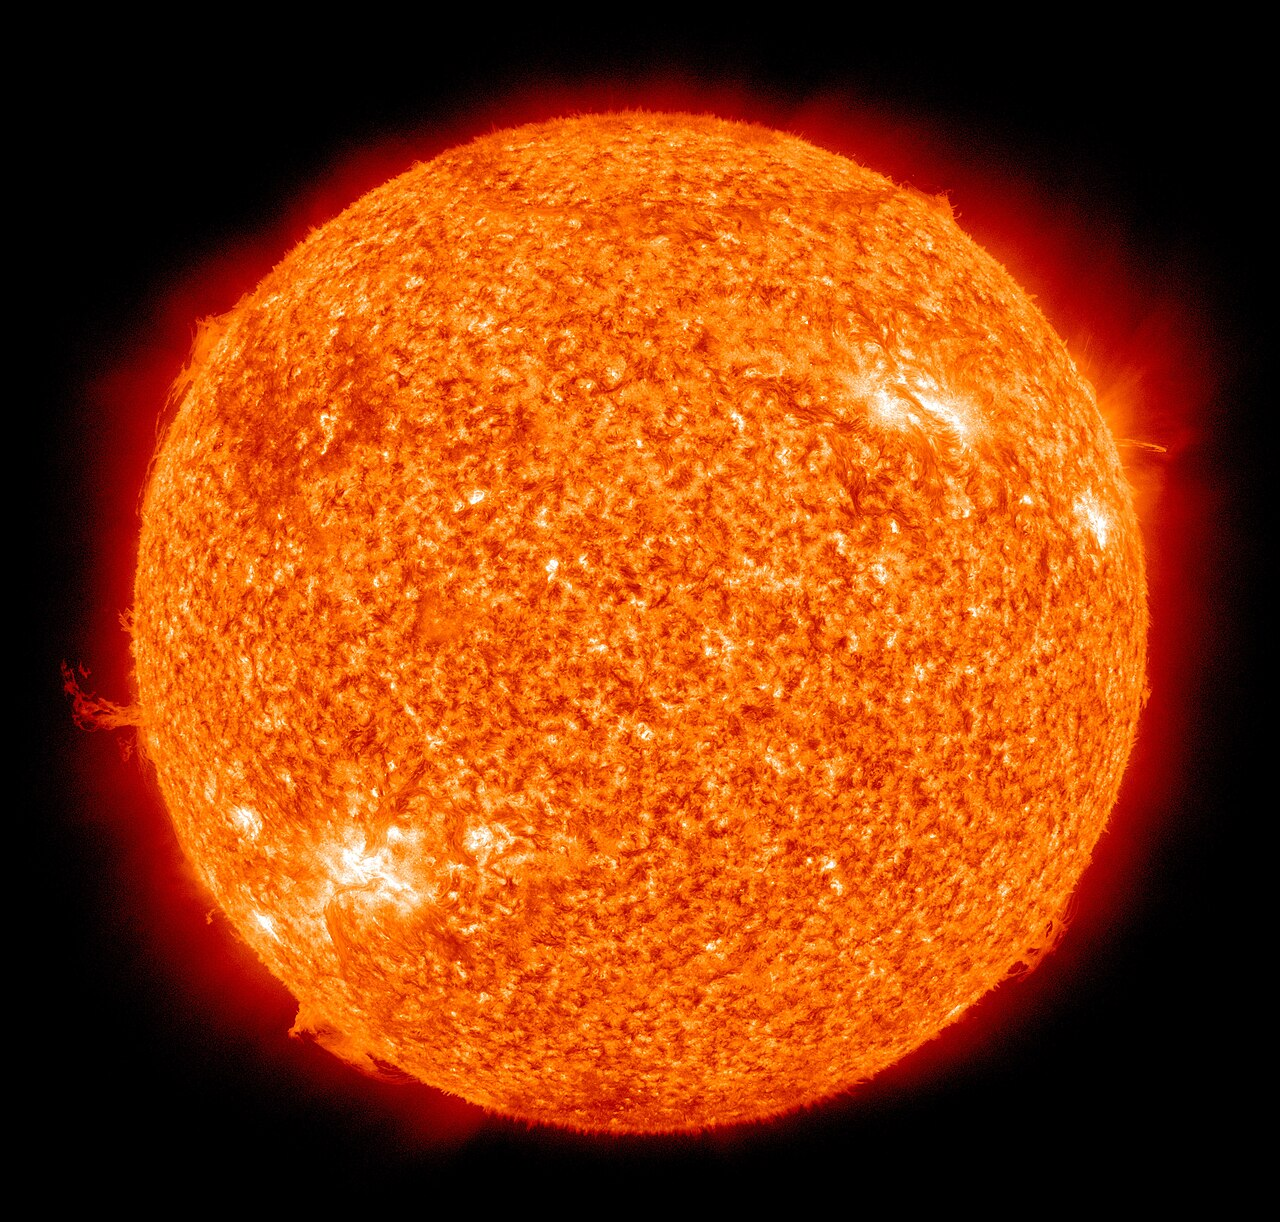
\includegraphics[width=0.4\linewidth]{images/book4/sun-sdo-aia.jpg}\hfill
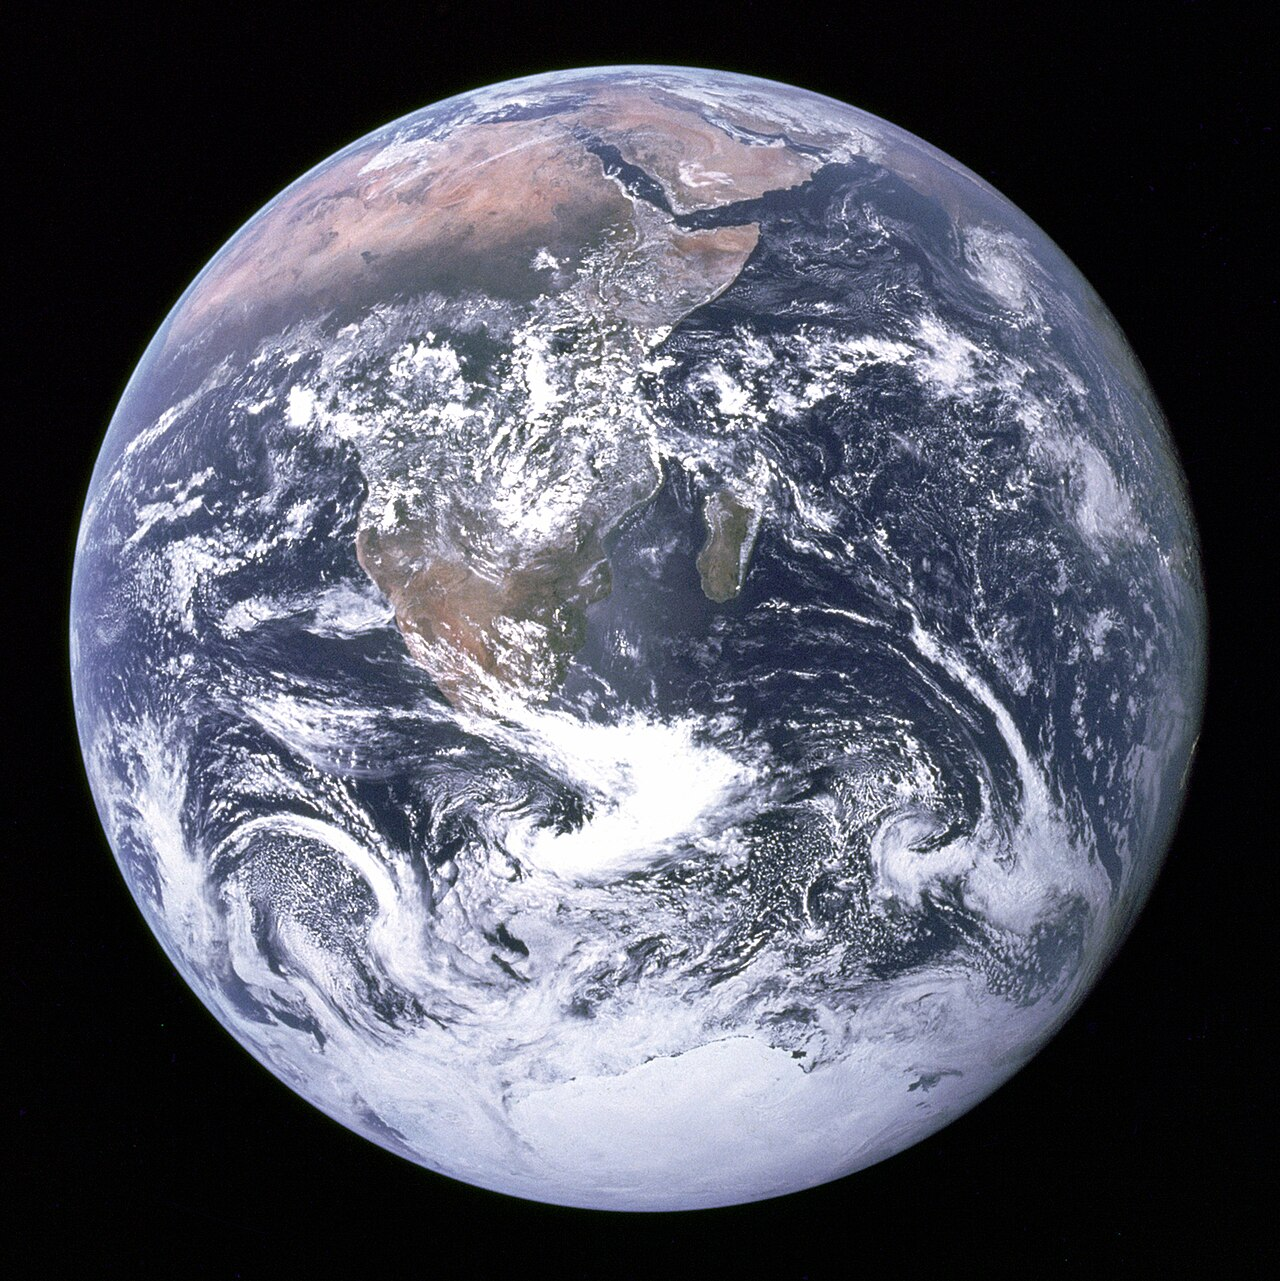
\includegraphics[width=0.4\linewidth]{images/book4/earth-apollo17.jpg}

{\small इस अध्याय की दोनों कृष्णिकाएँ: सूर्य, \qty{5800}{K} पर, जिसे सोलर डायनेमिक्स ऑब्ज़र्वेटरी ने चरम पराबैंगनी में देखा, और पृथ्वी, \qty{288}{K} पर, जिसका छायाचित्र अपोलो 17 के दल ने लिया --- और चोटियाँ \qty{0.5}{\micro m} तथा \qty{10}{\micro m} पर (NASA)।}
\end{omfigure}

\section{समस्या: पृथ्वी का ऊर्जा-बजट और तापदीप्त बल्ब}

\begin{problem}[{सप्ताहांत समस्या --- सूर्य से तंतु तक
कृष्णिकाएँ}]\label{pb:b2:thermal-radiation:1}
आँकड़े: $\sigma = \qty{5.67e-8}{W/m^2/K^4}$, $\lambda_{\max}T = \qty{2.90e-3}{m.K}$,
$h = \qty{6.63e-34}{J.s}$, $k_B = \qty{1.38e-23}{J/K}$, $c = \qty{3.00e8}{m/s}$;
सूर्य: $R_\odot = \qty{6.96e8}{m}$, $d = \qty{1.50e11}{m}$; पृथ्वी: $R =
\qty{6.37e6}{m}$, परावर्तांश $0.30$।

\textbf{भाग I --- \omterm{def:b2:thermal-radiation:blackbody}{कृष्णिका} की तरह सूर्य।}
\begin{enumerate}
  \item सौर वर्णक्रम की चोटी \qty{0.50}{\micro m} पर है: सतह का
        ताप।
  \item सतह का निर्गम और कुल ज्योति।
  \item पृथ्वी पर \omterm{prop:b2:thermal-radiation:earth}{सौर अचर}; और वहाँ धूप का ऊर्जा घनत्व तथा दाब।
  \item माध्य फ़ोटॉन ऊर्जा ($\approx 2.7\,k_BT$) और पृथ्वी पर प्रति सेकंड
        प्रति वर्ग मीटर सौर फ़ोटॉनों की संख्या।
  \item सूर्य $4.5 \times 10^9$ वर्षों से इसी दर पर विकिरित करता आया है:
        उत्सर्जित ऊर्जा; $Mc^2$ से तुलना कीजिए, $M = \qty{2e30}{kg}$ के लिए।
\end{enumerate}

\textbf{भाग II --- बिना वायुमंडल की पृथ्वी।}
\begin{enumerate}[resume]
  \item पृथ्वी से सोखी गई शक्ति; और \omterm{prop:b2:thermal-radiation:earth}{प्रभावी ताप}।
  \item संतुलन $4$ से क्यों भाग देता है? बिना घूमती, बिना हवा वाली
        पृथ्वी ($A = 0.30$) के अधःसौर बिंदु पर ताप
        क्या होता?
  \item चंद्रमा ($A = 0.12$): अधःसौर ताप; और उसका रात वाला
        पक्ष \qty{100}{K} तक क्यों गिर जाता है (दो-सप्ताह लंबे दिन के दौरान
        रेगोलिथ में संचित ऊष्मा के बारे में सोचिए, प्रभावी \qty{1e6}{J/m^2/K})।
  \item पृथ्वी के उत्सर्जन की चोटी का तरंगदैर्घ्य; सूर्य वाले से
        तुलना कीजिए।
  \item यदि और हिम या बादल परावर्तांश को $0.35$ कर दें, तो \omterm{prop:b2:thermal-radiation:earth}{प्रभावी ताप}
        कितना गिरेगा?
\end{enumerate}

\textbf{भाग III --- हरितगृह।}
\begin{enumerate}[resume]
  \item एक-परत प्रतिरूप के तीनों संतुलन (अंतरिक्ष, परत, सतह)
        लिखिए और $T_{\text{सतह}} = 2^{1/4}T_{\text{प्र}}$ पाइए।
  \item अवरक्त का अंश $\varepsilon$ सोखती किसी परत के साथ:
        $T_{\text{सतह}}(\varepsilon)$; और $\varepsilon$ का वह मान जो
        \qty{288}{K} दे।
  \item कौन-सी गैसें सोखती हैं, कौन-सी नहीं, और किस तरंगदैर्घ्य
        पट्टी में; और वायुमंडलीय खिड़की क्या है?
  \item $\varepsilon = 0.78$ वाले प्रतिरूप में वायुमंडल ज़मीन को जो अवरक्त
        लौटाता है, \unit{W/m^2} में; सोखी गई धूप से तुलना
        कीजिए।
  \item \qty{3.7}{W/m^2} का कोई प्रणोदन (दुगुनी कार्बन डाइऑक्साइड):
        बिना \omterm{def:b2:feedback-oscillators:loop}{पुनर्भरणों} के ताप-बदलाव $\Delta T = \Delta F/4\sigma T_{\text{प्र}}^3$।
  \item प्रति वर्ग मीटर \qty{50}{m} की महासागरीय मिश्रित परत की
        ऊष्मा-धारिता और उत्तर का समय-अचर।
  \item बादल सतह को ठंडा (परावर्तांश) भी करते हैं और गरम (अवरक्त) भी:
        रात में कौन-सा असर जीतता है?
\end{enumerate}

\textbf{भाग IV --- तापदीप्त बल्ब।}
किसी \qty{60}{W} बल्ब का टंग्स्टन तंतु \qty{2800}{K} पर है,
$\varepsilon = 0.35$; और किसी \omterm{def:b2:thermal-radiation:blackbody}{कृष्णिका} की शक्ति का जो अंश
दृश्य ($0.4$--\qty{0.7}{\micro m}) में पड़ता है वह \qty{2800}{K} पर $0.08$ और
\qty{3200}{K} पर $0.14$ है।
\begin{enumerate}[resume]
  \item तंतु का विकिरण करता क्षेत्रफल; उतना क्षेत्रफल रखते किसी
        \qty{50}{\micro m} तार की लंबाई; वह कुंडलित क्यों होता है?
  \item चोटी का तरंगदैर्घ्य; दृश्य शक्ति; और ज्योतीय दक्षता।
  \item \qty{230}{V} पर चलते तंतु का प्रतिरोध; कमरे के ताप पर
        टंग्स्टन की प्रतिरोधकता लगभग दस गुना छोटी है:
        चालू करते समय धारा, और उसका एक परिणाम।
  \item \qty{3200}{K} पर: उन्हीं \qty{60}{W} के लिए ज़रूरी क्षेत्रफल और
        दृश्य शक्ति; हर बल्ब \qty{3200}{K} पर क्यों नहीं चलाया जाता
        (टंग्स्टन की वाष्पन-दर हर \qty{50}{K} पर मोटे तौर पर दुगुनी हो
        जाती है)?
  \item हैलोजन चक्र क्या करता है, और वह किसी अधिक गरम तंतु की
        अनुमति क्यों देता है?
  \item \qty{60}{W} का बाक़ी कहाँ जाता है, और बल्ब का काँच
        \qty{150}{\celsius} तक क्यों पहुँच जाता है?
  \item बंद कर देने के बाद तंतु के ठंडा होने का काल: उसके द्रव्यमान
        (\qty{20}{mg}, $c = \qty{140}{J/kg/K}$) और उसकी विकिरित
        शक्ति से आँकिए।
  \item समेटिए: किसी \omterm{def:b2:thermal-radiation:blackbody}{कृष्णिका} का ताप क्या-क्या तय करता है, और
        तंतु, सूर्य तथा पृथ्वी में क्या साझा है।
\end{enumerate}
\end{problem}
